\section{Ambiente di lavoro}

Per il versionamento del codice e il coordinamento del gruppo è stato scelto di utilizzare \textbf{github}. Il progetto è stato infatti inserito e gestito all'interno di una repository \texttt{git}, in modo da controllare ogni singola modifica e rendere cooperativa la scrittura del codice.

Inoltre, per l'assegnazione dei task e il rilevamento dei bug è stato utilizzato il sistema di gestione delle \textit{issues}, che permette di gestire in modo molto efficace e ordinato il tutto, attraverso l'assegnazione ai vari membri e al filtraggio tramite le etichette.

\begin{figure}[H]
		\centering 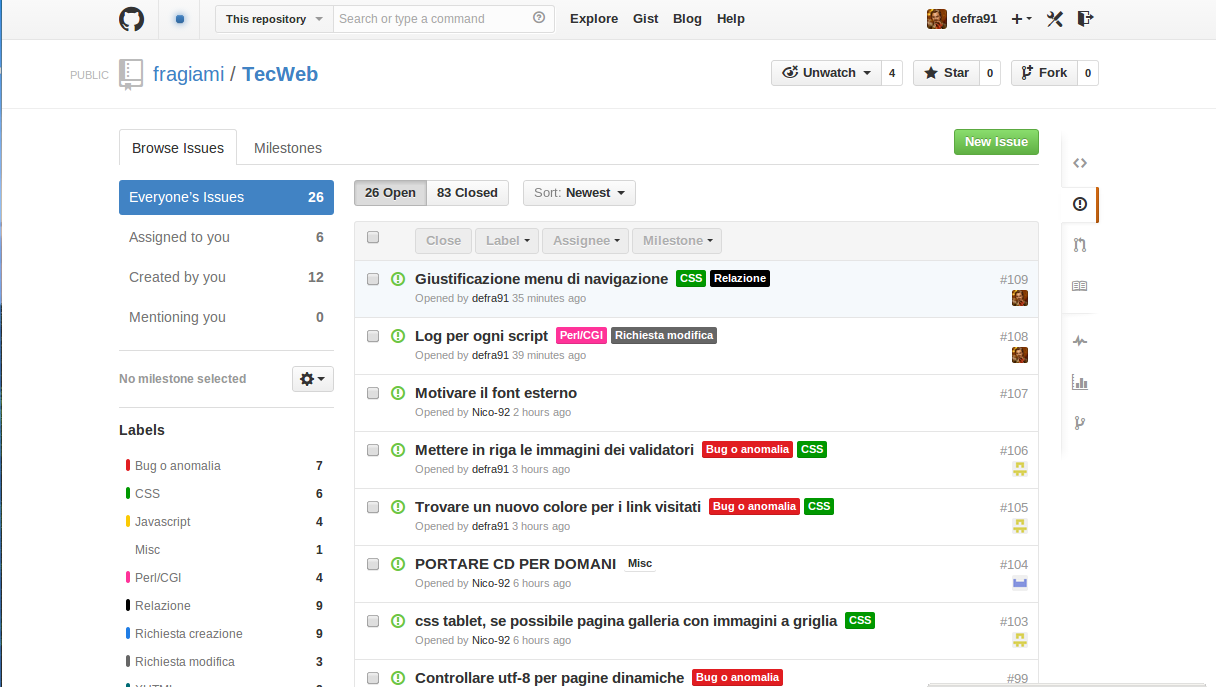
\includegraphics[width=0.8\textwidth]{images/github.png}
		\caption{Visualizzazione delle issues di github}
\end{figure}


